\section{Linked Data}
One of the most critical aspects of the Semantic Web is the ability to create links between multiple datasets. These links are described in a standardized framework, RDF, as previously described in \Cref{ssec:formatting-RDF}. Not only do these links allow humans to traverse the web, but they also provide a similar pathway for machines to traverse the web as well.\\

\noindent To qualify as Linked Data, the following four conditions need to be met \cite{bizer2011linked}:

\begin{enumerate}
    \item Objects have to be identified through a unique resource identifier (URI).
    \item These URIs have to be HTTP URIs.
    \item Data has to be found when we follow such a URI. This data can be formatted in many ways, such as XML.
    \item The data has to include links to other data. These links are vital to establishing a ``web'' of data.
\end{enumerate}

\noindent A simple way to represent Linked Data is by using a directed graph, such as visualized in \Cref{fig:LinkedData}. In this figure, the vertices represent objects or data points, whereas the edges represent the links that connect objects or data points. Among other things, this example visualizes the aforementioned \texttt{Alice - Knows - Bob} relation. Additionally, the object Alice has a \texttt{Name}-link to a data point with the value ``Alice''. From this, we can infer that the name of the object is Alice.\\

\noindent Finally, observe that every object has at least one link, which implies a connected ``Web of Data''.

\begin{figure}[htbp!]
    \centering
    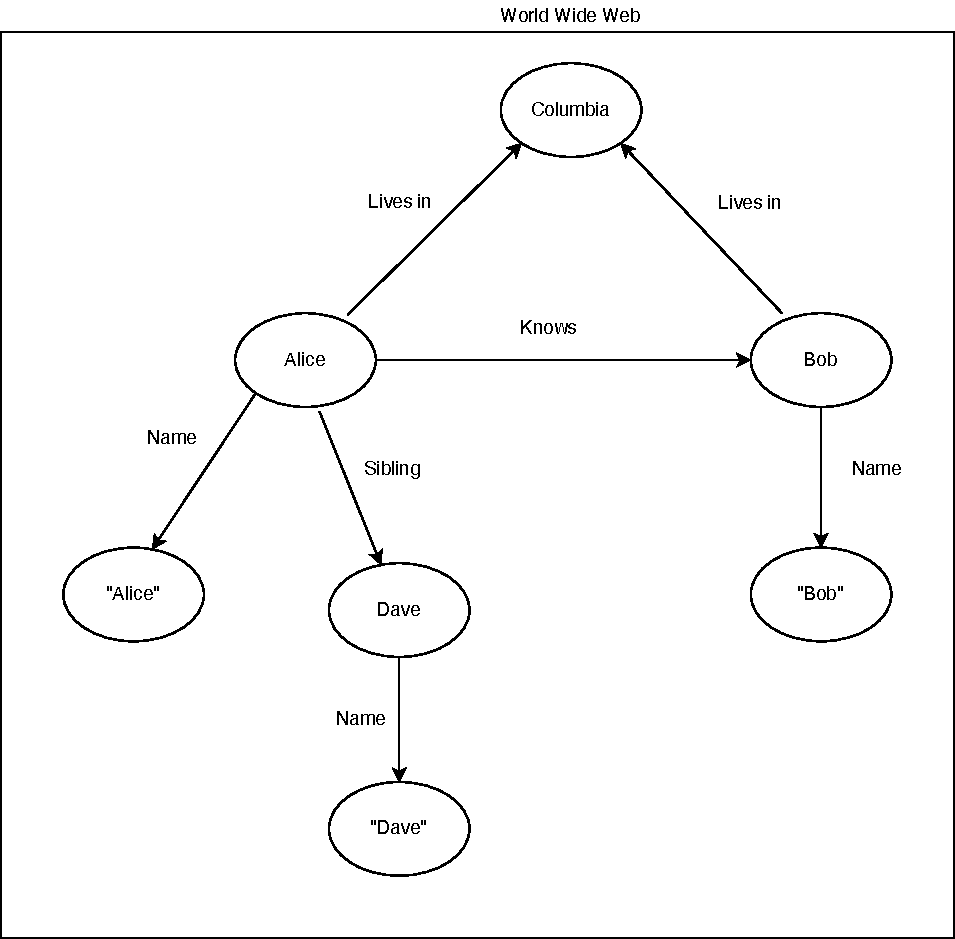
\includegraphics[width=\textwidth]{images/linked-data.pdf}
    \caption{Example of a linked data web.}
    \label{fig:LinkedData}
\end{figure}

\subsection{SPARQL}\label{ssec:sparql}
SPARQL \cite{world2013sparql} (a recursive acronym that stands for the SPARQL Protocol and RDF Query Language) is a semantic query language that allows to query and edit data stored in the RDF format. It is the standard query language for RDF and was adopted by W3C\footnote{\url{https://www.w3.org/blog/SW/2008/01/15/sparql_is_a_recommendation/}} as a recommendation in 2008. SPARQL is similar to SQL\footnote{\url{https://www.w3schools.com/sql/sql_quickref.asp}}, but where SQL operates on relational databases, SPARQL operates on the Semantic Web. While the functionality is not completely the same, the style of querying for information is very similar, as shown in \Cref{lst:sparql-example}.

\lstinputlisting[caption={SPARQL example that lists the names of all the objects that have this link, from W3.org (\url{https://www.w3.org/2009/Talks/0615-qbe/}).},label=lst:sparql-example]{snippets/sparql-example.txt}